\documentclass[a4paper,12p]{article}
\usepackage{standalone}
\usepackage{polski}
\usepackage[utf8]{inputenc}
\usepackage{amsmath}
\usepackage{physics}
\usepackage{amsfonts}
\usepackage{mathtools}
\usepackage{algorithm}% http://ctan.org/pkg/algorithms
\usepackage{algpseudocode}% http://ctan.org/pkg/algorithmicx
\usepackage{tikz}
\usepackage{amssymb}
\usepackage{indentfirst}
\usepackage{amsthm}
\usepackage{hyperref}
\usepackage{float}
\linespread{1.5}

\renewcommand{\refname}{Źródła}
\newcommand\tab[1][1cm]{\hspace*{#1}}

\begin{document}

\begin{titlepage}
	\begin{center}
	
	{\huge\bfseries Algorytmy zaawansowane - raport z projektu} \\
	\vspace{1cm}
	{\Large\scshape Wiktor Gontarczyk\par}
	{\Large\scshape Tomasz Laskowski\par}
	\vspace{2cm}

	\today
	\vspace{1cm}	
	
	\end{center}
\end{titlepage}

\section{Przypomnienie - cel projektu}

Celem projektu było znalezienie i zaimplementowanie algorytmu rozwiązującego problem znajdowania drzewa dla podanej macierzy odległości pomiędzy jego liśćmi. Zdecydowano się na algorytm opierający się na znajdowaniu kodu Prüfera.

\section{Instrukcja obsługi}

Program został zaimplementowany w języku Python, dostępny jest zarówno oryginalny skrypt, jak i wykonywalny plik .exe, utworzony przy użyciu biblioteki \texttt{pyinstaller}. Program jest aplikacją konsolową i oferuje dwie możliwości podania parametrów: przez plik csv oraz bezpośrednio z konsoli. Jedynym potrzebnym argumentem jest macierz odległości ozn. w algorytmie jako macierz $D$.

Macierz jest poddawana walidacji: powinna być symetryczna z zerami na głównej diagonali. W przypadku podania niepoprawnych danych program wypisuje błąd. W przypadku powodzenia wypisane zostaną: sekwencja Prüfera oraz słownik z listowym zapisem otrzymanego drzewa (kluczami są numery wierzchołków, a wartościami listy sąsiadów).

Aby podać dane przez plik, należy zapisać macierz w klasycznym dla pliku csv formacie: wiersze oddzielając znakiem nowej linii, natomiast kolejne elementy wiersza przecinkami (przykład w wysłanym rozwiązaniu). Wywołujemy program z flagą \texttt{--file} (\texttt{-f}), jako argument podając ścieżkę do pliku.

Przykład:

\texttt{./az-tree.exe --file ./tree.csv}

Aby podać dane bezpośrednio w konsoli należy zapisać macierz w formie dwuwymiarowej listy, zgodnie z syntaktyką języka Python. Argument powinien zostać ujęty w cudzysłów. Do tego wywołania służy flaga \texttt{--distances} (\texttt{-d}).

Przykład:

\texttt{./az-tree.exe --distances "[[0, 2, 3], [2, 0, 3], [3, 3, 0]]}

Program posiada również dodatkową opcję rysowania znalezionego drzewa, bardzo pomocną przy implementacji i testach. Służy do tego flaga \texttt{--output-file}, a jako argument podajemy nazwę wynikowego pliku (w formacie PNG). \textbf{Uwaga:} ta metoda wymaga zainstalowania pakietu Graphviz.

Przykład:

\texttt{./az-tree.exe --file ./tree.csv --ouput-file ./tree.png}

Inną opcją uruchomienia algorytmu jest podanie parametrów drzewa do wylosowania: liczby wierzchołków n, oraz liczby liści l jako parametr \texttt{--random-tree} w formacie n:l. Wtedy użyta zostanie macierz odległości pomiędzy liśćmi wylosowanego drzewa. 
W przypadku gdy wybrano opcję rysowania drzewa, zostanie dołączone także drzewo wejściowe jako plik o nazwie \verb$original-<nazwa_pliku_wyjściowego>$. 
Dodatkową opcją jest sprawdzenie czy drzewo wejściowe jest izomorficzne z drzewem zrekonstruowanym przez algorytm. Służy do tego flaga \texttt{--test-isomorphism}.

Przykład:

\texttt{./az-tree.exe --random-tree 100:20 --ouput-file ./tree.png}

Lub z włączonym testem izomorfizmu:

\texttt{./az-tree.exe --random-tree 100:20 --ouput-file ./tree.png --test-isomorphism}

Skrót powyższej instrukcji w formacie Markdown jest również dostępny wśród wysłanych plików.

\section{Zmiany w stosunku do planu}

W stosunku do planu ze wstępnej dokumentacji oraz późniejszych, zgłoszonych poprawek zaszło kilka zmian w samym algorytmie:

\begin{enumerate}
	\item Początkowo zamierzono zrezygnować ze zbioru ozn. $S$, jednak okazało się, że dla metody z wyszukiwaniem jednego liścia na raz, algorytm nie działa poprawnie w niektórych przypadkach - nie udało się przez to zmniejszyć złożoności.
	\item Poprawiono niepoprawny warunek zakończenia głównej pętli (drobny błąd w zapisie algorytmu).
	\item Poprawiono funkcję odpowiadającą za wyszukiwanie liści.
\end{enumerate}

\section{Testy}

\subsection{Testy poprawności implementacji algorytmu}

W pliku tests.py załączono testy algorytmu na ręcznie zweryfikowanych przykładach. Wykorzystano również testy z użyciem losowego wygenerowania macierzy odległości pomiędzy liśćmi dla drzewa wejściowego o liczbie wierzchołków z zakresu od 4 do 80 z krokiem 4 i o losowej liczbie liści. W tym przypadku sprawdzano izomorfizm grafów. Testy poprawności przebiegły pomyślnie.


\subsection{Testy wydajnościowe algorytmu}

Przeanalizowano wydajność algorytmu wykorzystując losowe generowanie drzew o zadanej liczbie wierzchołków i liści. Dla danej liczby wierzchołków w zakresie od 10 do 600 z krokiem 10 i zmiennej liczby liści z zakresu od dwóch do $n-2$ interpolowanej liniowo z krokiem 5 (długość sekwencji) zmierzono czasy wykonania algorytmu i uśredniono. Wyniki zapisano w pliku benchmark.csv, wygenerowanym skryptem benchmark.py.
Uśrednione dla każdego n czasy wykonania algorytmu przedstawiono na poniższym wykresie.

\begin{figure}[H]
    \centering
    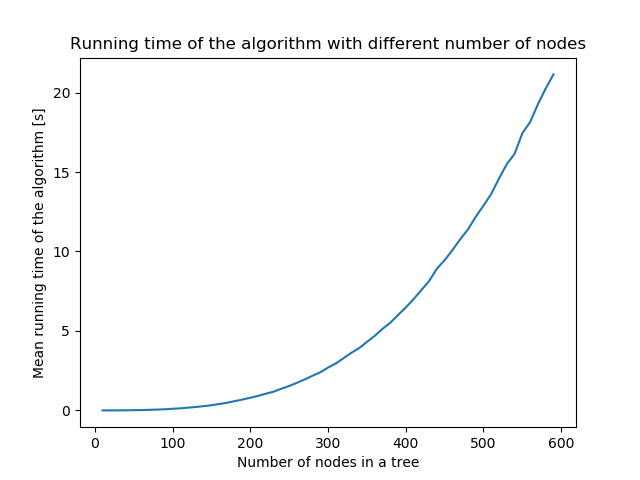
\includegraphics[width=.9\textwidth]{benchmark.png}
    \caption{Wykres czasu wykonania algorytmu w sekundach w zależności od liczby wierzchołków drzewa.}
    \label{fig:mesh1}
\end{figure}

Wyniki można powtórzyć wywołując skrypt benchmark.py.

\section{Podział pracy}

Wiktor Gontarczyk - implementacja, testy, pomiary czasowe, dowód poprawności

Tomasz Laskowski - implementacja, testy, przygotowanie pliku wykonywalnego, instrukcja obsługi, opis algorytmu, złożoność.

\end{document}